\chapter{Literature Review}
This section reviews various academic sources related to the methodology proposed. It will look at the various fields of engineering as well as biomechanics to form a holistic understanding of the design space. Importantly the technologies discussed will also be related to the field of robotics as  




\section{Introduction}
This research project brings together various disciplines of research. By combining techniques from computer vision, sensors and data fusion we can design and develop new way of capturing human gait data. Whilst the fields of biomimicry and bio-inspired robotics are relatively new, recent advances in related fields such as artificial intellegence and computer vision have invigorated the persuit of functional humanoid robotics. 

Humanoid robotics \cite{kaneko2002design}   ... talk about dynamics...






\section{Human Motion and Gait}
The human gait is well understood and has been studied in detail as it is a fundamental part of human mobility. It is one of the first skills developed in infancy and its importance for healthy develpoment, as outlined by Adolph et al. \cite{adolph2013road}, cannot be understated. Walking and running are also critical factors in transportation and geographical movement of people and goods in developing countries where public transport is underdeveloped and private transport not within the means of the populous. Finally walking and running as exercise has proven benefits as shown in \cite{hanson2015there} (general health) and \cite{fox1999influence} (mental health).     

There is thus clear evidence that the human gait has earned its right as a field of study in academia.









\section{Computer Vision}
While the previous section answers "why" understanding the human gait is important, the following sections will explain fields that contribute to the question of "how" the gait is studied. The technologies used and the 

Computer vision is a field borne from image processing and artificial intelligence that seeks to replicate the ability of the human visual system.   







\subsection{Computer Vision in robotics}
Recent improvements to real time computer vision has allowed amazing technological breakthroughs in fields closely related to robotics. One such breakthrough is the rapid improvement of self-driving cars developed by Tesla. These vehicles use vision based technologies and real time image processing to navigate complex and changing road networks. 

Furthermore 










\subsection{New Perspectives from Animal Borne Cameras}
Patel et al. \cite{patel2017trackingieee} showed that using animal borne cameras and motion sensors, the tail kinematics of the cheetah (Acinonyx Jubatus) could be tracked. Patel's work was partly inspired by Kane et al. \cite{kane2014falcons} where falcon (Falco Peregrinus) borne cameras were used to better understand airborne pursuit of prey. Giving researchers a new perspective on the behaviour of animals in the natural world.

Further work completed by Pearson et al. \cite{pearson2017testing} showed that cameras mounted to dolphins (Lagenorhynchus Obscurus) could provide insight into the their movement, social and foraging strategies. Using cameras to study ocean-life has become a popular methodology in recent time due to difficulties imposed by their environment. In essence We struggle to understand flying and swimming animals due to their complex environments.   









\subsection{Human Motion Analysis Using Computer Vision}
From Chen et al.\cite{chen2013survey} using depth imagery to understand human motion we can see that this is a popualr teqnique. 














\section{Inertial Measurement Units and Sensors}
IMU's are a staple of electrical engineering as applied to dynamic systems. These sensors give us insight as to how an object is moving in space by providing data relating to orientation and acceleration of said system. These data points are created by electronically interpreting signals generated by micro-electromechanical system (MEMS). Modern smartphones have built in IMU's that are not only accurate \cite{gikas2016rigorous}, but also easy to interface with due to the open source nature of the Android operating system \cite{androidSensorLib}.  

Generally Smartphones contain the following sensors:
\begin{itemize}
\item Accelerometer
\item Gyroscope
\item Magnetometer
\item Barometer
\item Temperature
\end{itemize}

\textbf{Accelerometers} provide linear acceleration data; these accelerations may be constant (eg. gravity) or changing (eg. relative motion). In smartphones they are usually based on MEMS that use  

\textbf{Gyroscope} provide rotational data relative to the sensors body. They provide angular accelerations 

\textbf{Magnetometers} provide information realting to the macroscopic magnetice fields surrounding the earth

\textbf{Barometers} are finely tuned atmospheric pressure sensors that can determine the relative height of an object with respect to sea-level.

\textbf{Temperature} generate local temperature data 





\subsection{Inertial Measurement Units in Robotics}
IMUs are integral in the functioning of robotics. Up until very recently intellegent robotic systems  had no sense of vision to provide feedback for their internal control systems. Instead this feedback was generated by various sensors providing information about the dynamics of these systems.










\subsection{Human Motion Analysis Using Inertial Measurement Units}
\cite{picerno201725}










\section{Mathematical Modelling}
The binding element presented in this work is the underlying mathematics. Using various mathematical tools and methods known to robotics and biomechanics it is possible to transform various datatypes in various frames of reference to a singular model.








\subsection{Mathematical Models of the Gait}
Before exploring complex methods and tools it is important to select and understand the model used.

Due to the large amount of existing research related to the human gait some models have been well established. These models are capable of quantifying important elements of the human gait. A popular model of choice is the multi segmented model 

Some fundamental work complete by Zajac, Neptune and Winters

\cite{zajac1990modeling} 
interesting to note the how he compared modelling difficulties to that seen in robotics..

\cite{zajac2002biomechanics}


\cite{zajac2003biomechanics}


collection of rigid beams


\subsection{Linear Kinematics}
By using kinematics we can quantify and understand the movement of the lower limbs. Kinematics is a branch of mechanics that fully defines the motion of a point with respect to position, velocity and acceleration (be it linear, rotational or a combination). Kinematics does not however describe the forces, torques or other variables that may affect that point. This is due to a fundamental assumption in kinematics that the point is massless.	 

Kinematics can be broken up into 2 main branches: \textit{forward} and \textit{inverse}. To illustrate the matter the following diagram is that of a basic kinematic model.

\begin{figure}[!ht] 
\captionsetup{width=\linewidth, font=small}  
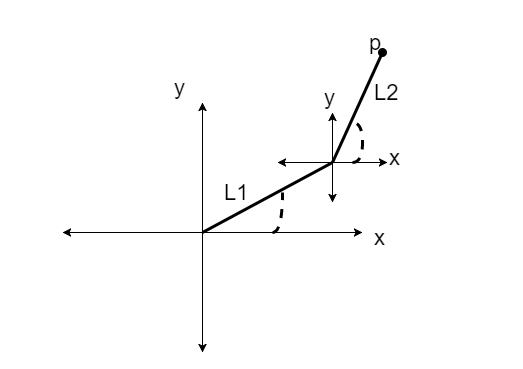
\includegraphics[width=\linewidth]{figures/kinematics.png}
\caption{Basic kinematic model to demonstrate}
\label{fig:kinematics}
\end{figure}

In this figure the position of point P is defined by 2 lengths, L1 and L2 with different lengths and angles from a set of shared axis. In forward kinematics we can find P if we know the angles and lengths of the different links in the system. The motion of point P can then be described by looking at  how the angles and lengths of the links in the system change over time.

Inverse kinematics uses knowledge of different points in the system, such as the origin and P and the lengths of the links in the system to determine the angular offsets of each length. Since these produce a set of linear equations, the more unknowns we are faced with the more possible solutions we can generate.

As discussed in the previous section a common method of modeling the human lower limbs is to use a collection of rigid beams. 


\subsection{Rotational Matrices}
There is an underlying difficulty in mathematically fusing various data sources and models; that of finding a common frame of reference. With the intent of using Lagrangian mechanics good definitions for the different frames are critical. This thesis will primarily use 2 different frames of reference. The inertial frame and the body frame.

The inertial frame (or world frame) can be defined in different ways as seen in \cite{soechting1992moving}, for the these NED (North East Down)	.

Rotational marices are mathematical objects that rotate vectors.
Since most engineering is constrained to the physical three dismensional world these matrices commonly rotate 3 dimensional vectors. 

This is an old problem ask euler.











\subsection{Kalman FIlter and Extended Kalman FIlter}
The Kalman filter is a mathematical tool used to estimate the states of a system using joint 

Kalman filters can be broken down into 2 fundamental stages of operation; a prediction and measurement stage. The prediction stage esentially takes the known currernt states of the system and estimates what the measurements should be for the next time interval. The measurement stage takes in measurements and mathematically detemines the states.

The states of the system are user defined parameters that can often not be directly measured.

Closely related to the field of control engineering the kalman filter proves problematic when applied to nonliner systems. From this was born the extended Kalman filter used to beter apply to nonlinear systems

an important elementto understand of these systems is as control engineers define the cost function. Within the field of optimal control we wnat to control system ebhavious using minial inpu and with minimal error. the cost function is a mathematical representation of these extremes.. 

















\section{Observing Natural Solutions for Robotic Shortcomings}
Naturally the question arises:  why would we want to better understand the dynamics of animals? A persistent problem in the field of modern robotics is that of mobility; robots struggle to navigate real world surfaces and obstacles. Work by Patel et al. \cite{patel2013rapid} shows how we can look towards nature for inspiration to solve this mobility problem. 

As demonstrated by various prototype robots built by Boston Dynamics bipedal robots are severely limited in manoeuvrability when compared to   















\section{Conclusion}
This chapter has shown the direct pararels of technologies related to gate capture to dynamic robotic systems. With these strong parllels in mind the transferability of these systems from humans to humanoid robots is clear.

ust as we can see the relatoipn work on the human body has to that of robotics we can use engineering methods developed for mechanical systems to understand complex ystems such as the human body.



































